\chapter{General Features}

\section{Sharing}
A Shareable Container or Item or Note can be shared with other user(s). An entity that needs to be shared has to be tagged as Shareable when it is created. This is because a Private entity cannot be shared.

\section{Revoking Sharing}
The sharing of a Container/Item/Note can be stopped by revoking. When the sharing is revoked, the recipient(s) will no longer have access to the shared entity.

\section{Expiring Sharing}
It is possible to set an expiration date on the sharing of a Container/Item/Note. After the expiration date, the expired entity will not be visible to anyone other than the owner. The expiration date can be changed at will by the owner of the entity.

\section{Granting Permissions}
The owner of a Container/Item/Note can share it with another user. When it is shared, the recipient will get
only permission to 'view' the artifact. The owner can grant two special permissions to the recipient. One is 'update' and the other is 'own'. When the recipient is granted update permission, the recipient can edit the artifact. If the recipient is granted 'own' permission, then the recipient can take ownership of the artifact. Once the ownership is taken over by the recipient, the original owner will only have view permissions.

There are some features and menus that are commonly available in various screens in Obidos. 
These are outlined here for easy reference.

\section{Help Menus}
\subsection{Top Level Menus}
There are 6 top level menus in Obidos. They are Notes, Items, Containers, Templates, Groups and History. 
Each of these top level menus has a Help selection. This Help page covers aspects of operations 
within that top level menu at a high level.

As an example, looking at the Notes top level menu, there is a Help menu for Notes (see following Figure).

\begin{figure}[H]
\centering
\fbox{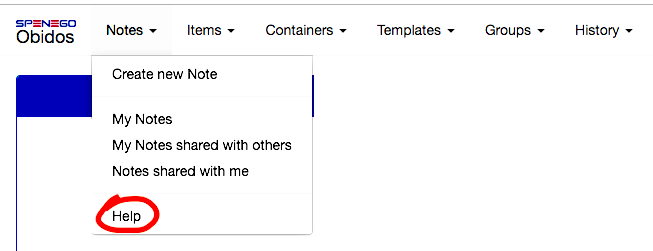
\includegraphics[scale=0.35]{user/Note-Help.png}}
\caption{Main Help for 'Notes' top level menu}
\label{fig: Figure}
\end{figure}

Similarly, for the Containers top level menu, there is a Help menu for Containers.

\begin{figure}[H]
\centering
\fbox{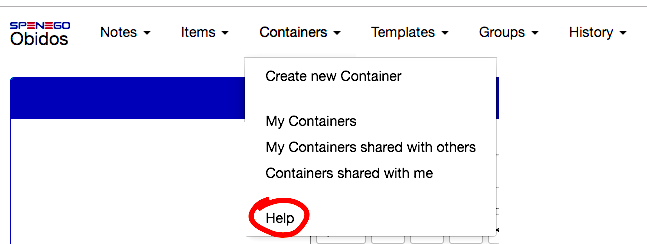
\includegraphics[scale=0.35]{user/Container-Help.png}}
\caption{Main Help for 'Containers' top level menu}
\label{fig: Figure}
\end{figure}

\subsection{Screen Level Menus}
Every screen has a Help section.
This Help section is accessible by clicking on the 'Help' button at the right of the blue header bar.
(See the red circled area in the following Figure).

\begin{figure}[H]
\centering
\fbox{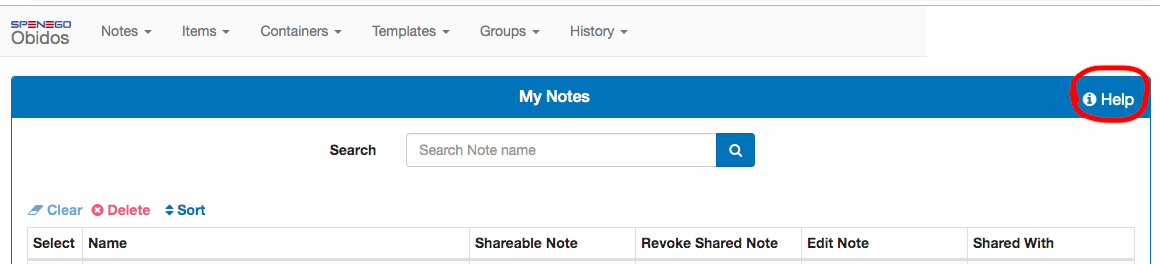
\includegraphics[scale=0.35]{user/List-Notes-Help.png}}
\caption{Screen level Help}
\label{fig: Figure}
\end{figure}

This screen level Help is a toggle button. When you click on the Help button, the help section will
open up at the top of the page. Clicking on the Help button again will collapse the help section. 

\section{Action Icons}

In many of the sections to follow, you will come across the following icons. Each one of these icons represent
a specific action that can be performed on the artifact in context. 
Some icons are reused in different scenarios with different colors.
These icons are listed here for easy reference.
\newline

\begin{center}
    \begin{tabular}{ | c | c | c | }
        \hline
        \textbf{Icon} & \textbf{Meaning} & \textbf{Description} \\
        \hline
            {\color{mygreen}\faPlusCircle} & Add & Add an Item to Container \\
        \hline
            {\color{myblue}\faEraser} & Clear & Clear the selections made \\
        \hline
            {\color{red}\faTimesCircle} & Delete & Delete the selected entities \\
        \hline
            {\color{orange}\faEdit} & Edit & Edit the entity in context \\
        \hline
            {\color{red}\faClockO} & Expired & This Note or Item has expired \\
        \hline
            {\color{red}\faEyeSlash} & Hide & Hide the Note or Item currently viewed \\
        \hline
            {\color{myblue}\faUsers} & List & List users and groups the entity is shared with \\
        \hline
            {\color{mygray}\faBan} & None or Not Allowed & The current activity in context is Not allowed \\
        \hline
            {\color{red}\faUnlock} & Not Secure & Value of this field is stored in plain text \\
        \hline
            {\color{mygray}\faLock} & Private & This entity is tagged as Private \\
        \hline
            {\color{orange}\faBan} & Revoke & Revoke sharing the entity in context \\
        \hline
            {\color{mygreen}\faLock} & Secure & Value for this field is stored encrypted \\
        \hline
            {\color{myblue}\faShareAltSquare} & Share & Share this artifact with others \\
        \hline
            {\color{mygray}\faShareAlt} & Shareable & This entity is tagged as Shareable \\
        \hline
            {\color{myblue}\faShareSquare} & Shared & Shows that the entity is shared with some user(s) \\
        \hline
            {\color{myblue}\faSort} & Sort & Sort the list of entities \\
        \hline
            {\color{mygreen}\faEye} & View & View the currently hidden Note or Item \\
        \hline
            {\color{mygreen}\faClockO} & Will Expire & This Note or Item has an expiration set on it \\
        \hline
    \end{tabular}
\end{center}

\section{Lengths of Entries}

The following table summarizes the maximum number of input characters allowed when creating various entities.
\begin{center}
    \begin{tabular}{ | c | c | }
        \hline
        \textbf{Identifier} & \textbf{Max number of characters} \\
        \hline
            Name (Note,Item,Container etc.) & 64 \\
        \hline
            Template field & 32 \\
        \hline
            Comment field & 256 \\
        \hline
    \end{tabular}
\end{center}

\section{Navigation in Listings}

Navigation through the listing menus are similar and described here.
\newline
By default, the entities (Notes/Items/Containers/Templates/Groups) will be displayed in the order in which they were created with the latest one at the top.
To sort the list of entities in another order, click on {\color{myblue}\faSort} \textcolor{myblue}{Sort} icon above the list bar.
The sort menu will show up and you can sort based on those options.

\begin{figure}[H]
\centering
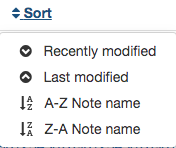
\includegraphics[scale=0.5]{user/Sort-Menu.png}
\caption{Sort Menu Options for Items}
\label{fig: Figure}
\end{figure}

The number of entities that exist can be seen at the bottom of the screen.
For example if there are 23 entities and 14 are listed in the current screen, at the bottom of the screen you will see 

\begin{center}
{\color{myblue}\faStepBackward} {\color{myblue}\faChevronCircleLeft} 1-14 of 23 
{\color{myblue}\faPlayCircle} {\color{myblue}\faStepForward}
\end{center}

In order to move forward in the list one at a time, click on {\color{myblue}\faPlayCircle}.
To move forward a complete page, click on {\color{myblue}\faStepForward}.
Similary, to go back in the list one at a time, click on {\color{myblue}\faChevronCircleLeft}.
and to go back one complete page, click on {\color{myblue}\faStepBackward}.
